\documentclass[10pt,twocolumn,letterpaper]{article}

\usepackage{iccp}
\usepackage{times}
\usepackage{amsmath}
\usepackage{amssymb}
\usepackage{url}
\usepackage{graphicx}
%\usepackage[backend=biber,style=ieee,sorting=ynt]{biblatex}

\newcommand{\cecilia}[1]{\textcolor{red}{cecilia: #1}}
\newcommand{\jinkyu}[1]{\textcolor{blue}{jinkyu: #1}}
% for rapid builds, with bounding boxes instead of images add the [draft] option to graphicx
% \usepackage[draft]{graphicx}

%\iccpfinalcopy % *** Uncomment this line for the final submission

%\addbibresource{vcd.bib}

\def\iccpPaperID{****} % *** Enter the ICCP Paper ID here
\def\httilde{\mbox{\tt\raisebox{-.5ex}{\symbol{126}}}}

% Pages are numbered in submission mode, and unnumbered in camera-ready
\ificcpfinal\pagestyle{empty}\fi
\begin{document}

%%%%%%%%% TITLE
\title{Draft: v0.5}

\author{
Jinkyu Kim\\
%{\small\url{http://www.author.org/~second}}
\and
Xuaner Zhang\\
{\tt\small cecilia77@cs.berkeley.edu}
\and
Ren Ng\\
%{\small\url{http://www.author.org/~second}}
}

\maketitle
\thispagestyle{empty}

%%%%%%%%% ABSTRACT
\begin{abstract}
   Abstract goes here. Place holder. Abstract goes here. Place holder. Abstract goes here. Place holder. Abstract goes here. Place holder. Abstract goes here. Place holder. Abstract goes here. Place holder. Abstract goes here. Place holder. Abstract goes here. Place holder. Abstract goes here. Place holder. Abstract goes here. Place holder. Abstract goes here. Place holder. Abstract goes here. Place holder. Abstract goes here. Place holder. Abstract goes here. Place holder. Abstract goes here. Place holder. Abstract goes here. Place holder. Abstract goes here. Place holder. Abstract goes here. Place holder. Abstract goes here. Place holder. Abstract goes here. Place holder. Abstract goes here. Place holder.
\end{abstract}

%%%%%%%%% Introduction
\section{Introduction}
\begin{figure*}
    \begin{center}
    \fbox{\rule{0pt}{2in} \rule{.9\linewidth}{0pt}}
    \end{center}
    \caption{Intro figure goes here}
    \label{fig:intro}
\end{figure*}

The era of an unprecedented ''myopic boom''~\cite{dolgin2015myopia} has been triggered around the world by a variety of environmental and behavioral factors. Half of young adult in the United States and Europe suffer from myopia, while up to 90\% of Chinese teenagers and young adults are shortsighted~\cite{dolgin2015myopia}. The prevalence of hyperopia has also been reported by various studies~\cite{yoo2013refractive, visionstudy}, 9.9\% and 11.6\% of populations ($\geq$40 years) respectively in the United States and Western European have hyperopia. 

Optical corrections (\ie, eyeglasses and contact lenses) have been primary options to correct eye's refractive errors. However, these corrections often cause inconvenience when people have to put them on and off based on their needs (\ie a person with hyperopia has to put on glasses whenever he/she wants to check time on a mobile phone). 

%Recent research~\cite{pamplona12,Huang:EECS-2011-162,huang14} has opened up a novel direction for computational vision correction: instead of correcting eye aberration from the viewer side, we could customize and correct the display to make it aberration compensated. When eye with defocus errors (\ie myopia and hyperopia) try to focus on a display outside its focal limit, their real focal planes lay closer (for myopia persons) or further (for hyperopia persons) than the display plane. If we could digitally refocus planes to the right position, which, in this case is the display plane, defocus could be corrected and viewers see the display in focus. Digital refocusing~\cite{ng2005light} and correction of lens aberration~\cite{ng2007digital} have been proposed for light field photography; similar idea to manipulate light field through ray tracing can be applied to build aberration compensated glassless light field displays. Previous works\cite{pamplona12,Huang:EECS-2011-162} have designed light field displays for vision correction, but their systems are view-dependent and undesired artifacts appear when the viewing point changes. In our system design, we account for eye movement so that the viewer is able to freely move within a viewing zone to see an aberration compensated display.

To alleviate this inconvenience, various techniques have been proposed [REF!], and recent works~\cite{pamplona12,Huang:EECS-2011-162,huang14} have opened up a novel direction for computational vision correction. These methods aim for manipulation of 4D light fields emitted by displays, while compensating optical eye aberration. However, there still remain concerns such as strong requirements that viewers should be placed in fixed viewing positions, otherwise undesired degradation of correction quality will be observed.

Here, we propose a novel framework for vision-correcting display that allows freedom in eye movements in the user-specified viewing zone, providing continuous viewing environment. Inspired by the idea of digital refocusing~\cite{ng2005light}, 4D light fields coming to the viewing zone from the virtual plane are rendered and displayed through light field displays. The location of virtual plane is determined by where images come to focus on retinal plane for myopic and hyperopic eyes.

The rest of the paper is organized as following: in the next section, we will have a review of light field display and its application to vision correction. Then we present general vision correcting display design and our proposed design. An analysis regarding viewing zone, limitation of defocus correction and display resolution is discussed afterwards. Then we show some simulation results with discussion and future work at the end.


\subsection{Contributions}
We propose a novel framework for vision-correcting display to free eye-movement within a specified viewing zone, while compensating for low-order optical eye aberration (\ie, myopia and hyperopia). We summarize our contributions as follows:

\begin{itemize}
\item We propose a framework for vision-correcting display that captures light field of a virtual image placed at eye’s focal plane. Light rays entering a viewing zone are represented by the light field signal so that viewing point is free to move within the viewing zone to view the display in focus.
\item We explore a design space to build a view-independent vision correcting display, providing trade-offs among size of viewing zone, of virtual image, and of the display. An analysis of minimum spatial and angular resolution requirements of the display to compensate for low-order eye aberration is also presented.
\end{itemize}


%-------------------------------------------------------------------------
\section{Related Work}
\subsection{Light Field Displays}
In a light field display system, a light field signal that characterizes how rays transport in a 3D virtual scene is displayed to the viewers. Viewers see these incoming light rays converged at different depths, as if emitted from objects at certain depths. Recent works ~\cite{ranieri2012multi,wetzstein2012tensor,maimone2013focus} in automultiscopic display have focused on using dual or multi-stacked LCD to realistically reproduce depth cues such as focus cue, motion parallax and binocular cues.

If we fix the focal plane at depth $\mathcal{D}$ and make the light field signal only capture a slice of the 3D virtual scene at depth $\mathcal{D}$, then the viewer with a good sight will see the 2D virtual plane in focus only when focal plane is at depth $\mathcal{D}$. Therefore, we can arbitrarily change the viewer's focal plane by properly modifying the light field signal that is put on the screen. This idea of tailored display is first introduced by Pamplona~\etal~\cite{pamplona12} to be applied to vision-correcting displays.

\subsection{Computational Vision Enhancement}

%Computational methods have been widely explored to enhance human vision, mainly in producing accurate depth cues when perceiving 3D scene geometry. Love~\etal~\cite{Love:09} uses fast switchable lens to form multiplexed image with nearly correct focus cue, and MacKenzie~\etal~\cite{mackenzie2010accommodation} introduces multiple‐-focal-‐plane display to improve vergence and accommodation conflicts. Instead of improving on producing depth cues such as vergence and accommodation, we use light field display to correct low order eye aberrations. Our vision-correcting display uses parallax barrier ~\cite{ives1903parallax}, in which a pinhole mask is placed in front of the liquid crystal display (LCD), to enhance focus ability for patients with low order eye aberration. Liu~\etal~\cite{liu2009time} creates a dynamic system that uses time-multiplexed dual-focal plane for head-mounted display, and a recent work by Itoh~\etal~\cite{Itoh:2015:VED:2735711.2735787} corrects defocus via overlaying a compensation image on the user's actual view to cancel the aberration for their head-mounted display. These methods, however, require external and moving parts. Another two vision-correction displays closely related to our work were presented by Pamplona~\etal~\cite{pamplona12} and Huang~\etal~\cite{huang14}, but both methods require a fixed viewing point, while we allow the eye to freely move within a viewing zone. A more in-depth comparison is discussed in section \ref{ss:vision-correcting-displays}.

\subsection{Vision-Correcting Displays}\label{ss:vision-correcting-displays}
Notable examples of utilizing light field displays to correct viewer’s optical aberration include works of Pamplona~\etal~\cite{pamplona12} and Huang~\etal~\cite{huang14}. Pamplona~\etal~\cite{pamplona12} introduced tailored display that uses 4D light fields to correct optical eye aberration with parallax-barrier and microlens arrays. Calculating pairs of display pixels and retinal sensors, a correction model is built to create decomposed virtual object placed on the viewer’s focal range. Following this framework, Huang~\etal~\cite{huang14} optimizes intensities of light fields with extended lateral viewing range, and shows improved reconstructed image quality on retina using a pin-hole mask.
 
These approaches, however, assume that viewer should be placed at a fixed lateral and axial position, leaving future work to incorporate eye-tracking techniques. Though Huang~\etal~\cite{huang14} provided an approach to optimize display values over multiple viewpoints, there are still challenging issues on resolving artifacts including cross-talks between two neighboring viewpoints, accurate estimation of viewer’s pupil size, and expensive computational cost to optimize over more viewpoints. In addition, Pamplona~\etal~\cite{pamplona12} provided reasonably fast algorithm for real-time system, but there are also unresolved artifacts (\ie, image jitter and screen flickering) when combined with eye-tracking techniques. In addition, bandwidth of display is not fully used, since pixel values are computed using a single viewpoint.



%-------------------------------------------------------------------------
\section{Designing Vision Correcting Display}

\subsection{Overview}
\begin{figure*}
    \begin{center}
        \fbox{\rule{0pt}{2in} \rule{.9\linewidth}{0pt}}
    \end{center}
    \caption{An system overview will be placed here}
    \label{fig:fig1}
\end{figure*}

\subsubsection{Eye Aberration}
An eye is in \textit{ametropic} condition when the relaxed eye fails to focus infinitely distant object on a focal point (\eg, retinal plane). The cause of ametropic includes changes in length of eyeball (\ie, distance between lens and retina) and abnormal changes in cornea or lens. Typical cases of \textit{ametropic} includes myopia (nearsightedness), hyperopia (farsightedness), presbyopia, and astigmatism.

In this paper, we focus on correcting low-order aberration (myopia and hyperopia). In-depth analysis on exploring high-order aberration is explained in Section~\ref{ss:Higherorderaberration}. A myopic eye often has too strong optical power for its axial length between the crystalline lens and the retina, making parallel rays from infinite distance come to focus on a point in front of the retina. The farthest point a myopic eye can focus on the retina is referred as the far point, and any image placed beyond the far point will appear blurred. Likewise, a hyperopic eye has too weak optical power and thus has its focal point behind the retina for parallel rays from infinity. The nearest point a hyperopic eye can focus on the retina is called a near point, and any image located in front of the near point will appear blurred.

\subsubsection{Correcting Low-order Eye Aberration with a fixed viewing position}
As illustrated in Figure~\ref{fig:overview}, we use 4D dual-plane light fields $L(u,v,x,y)$ to describe light rays from the lateral image plane ($uv$-plane) to the lateral eye's pupil plane ($xy$-plane). The incident light rays would focus on retina without any correction if the image is placed at the eye's far point ($P_f$, if myopia) or near point ($P_n$, if hyperopia). The incident light rays can be calculated by integrating rays coming to the eye's pupil.
\begin{equation}
	I(x,y) = \iint_{\Omega} L(u,v,x,y) dudv
\end{equation}
where $\Omega$ is limited by eye's entrance pupil. Now, let us consider a light field display that is placed in front of the viewer; for example, farther than the eye's far point (if myopia) or closer than the eye's near point (if hyperopia). If we denote $\tilde{L}(s,t,x,y)$ as two-plane light fields from the lateral display plane ($st$-plane) and the lateral eye's pupil plane ($xy$-plane), the incident light rays $\tilde{I}(s,t,x,y)$ can be derived as follows:
\begin{equation}
	\tilde{I}(x,y) = \iint_{\Omega} \tilde{L}(s,t,x,y)  dsdt
\end{equation}
The problem of correcting low-order eye aberration with a fixed viewing position is then fomulated as to find light fields $\tilde{L}^{*}$ that minimizes the following function:
\begin{align}
	\tilde{L}^{*} &= \text{argmin}_{\tilde{L}} \sum_{x,y} (I(x,y)-\tilde{I}(x,y))^{2}
\end{align}
This problem statement is consistent with previous works of Pamplona~\etal~\cite{pamplona12} and Huang~\etal~\cite{huang14}. 


%\begin{equation}
%	I(x,y) = \iint L(u,v,x,y)A(x,y)  dudv
%\end{equation}
%where $A(x,y)$ is a binary function limited by eye's pupil size.
%\[ A(x,y) =
%  \begin{cases}
%   0  & \quad \text{if $A(x,y)$ is placed inside the pupil}\\
%   1  & \quad \text{if $A(x,y)$ is placed outside the pupil}\\
%  \end{cases}
%\]
%Now, let us consider a light field display that can produce sufficient light fields, and is placed in front of the viewer: farther than the eye's far point (if myopia) or closer than the eye's near point (if hyperopia). If we denote $L'(s,t,x,y)$ as two-plane light fields from the lateral display plane ($st$-plane) and the lateral eye's pupil plane ($xy$-plane), the incident light rays $I'(s,t,x,y)$ can be derived as follows:
%\begin{equation}
%	I'(x,y) = \iint L'(s,t,x,y)A(x,y)  dsdt
%\end{equation}

%The problem of correcting low-order eye aberration with a fixed viewing position is then to find light fields $L'$ that minimizes $|I(x,y)-I'(x,y)|$ for any light rays coming to the eye's pupil. This problem statement is consistent with previous works of Pamplona~\etal~\cite{pamplona12} and Huang~\etal~\cite{huang14}. 

\subsubsection{Correcting Low-order Eye Aberration within viewing zone}
Now, let us consider the eye is moving in lateral direction on the pupil plane by $(\Delta x, \Delta y) \in R$, where  $R$ is the space satisfying following condition: $w_e/2 \leq \Delta x, \Delta y \leq  w_e/2$. We denote $w_e$ as the width of viewing zone where the viewer can freely move and see an displayed image without any reduction of perceived image quality. Now, the problem can be stated by finding light fields $\tilde{L}^{*}$ that minimizes the following function:
\begin{equation}
	\tilde{L}^{*} = \text{argmin}_{\tilde{L}} \sum_{R}\sum_{x,y} (I_{\Delta x, \Delta y}(x,y)-\tilde{I}_{\Delta x, \Delta y}(x,y))^{2}
\end{equation}
where $I_{\Delta x, \Delta y}(x,y)$ is $I(x-\Delta x,y-\Delta y)$.








\subsection{System Design}
In Figure~\ref{fig:overview}, we illustrate a 2D geometry of the proposed vision-correcting display for myopic eyes (top) and hyperopic eyes (bottom). The proposed framework consists of three planes: the light field display plane ($D$-plane), the virtual image plane ($V$-plane), and the eye's pupil plane ($P$-plane). Widths of each plane are denoted as: $w_d$ (for $D$-plane), $w_v$ (for $V$-plane), and $w_p$ (for $P$-plane), and these widths satisfy the following relationship:
\[ w_v =
  \begin{cases}
    (1-\alpha)w_l-\alpha w_p  & \quad \text{for myopia}\\
    (1+\alpha)w_l-\alpha w_p  & \quad \text{for hyperopia}\\
  \end{cases}
\]
where $\alpha$ is the ratio $d_v/d_e$, where $d_v$ and $d_e$ are distances from D-plane to V-plane and P-plane, respectively. 

\begin{figure}[t]
	    \begin{center}
		%\fbox{\rule{0pt}{2in} \rule{0.9\linewidth}{0pt}}
   		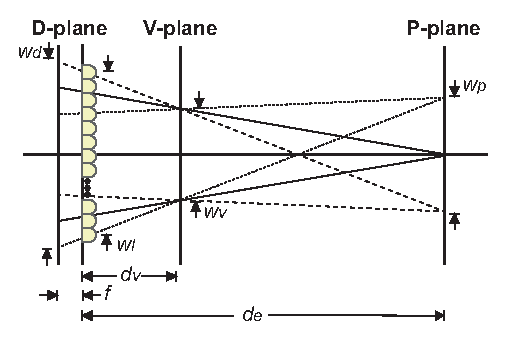
\includegraphics[width=0.95\linewidth]{images/overview_myopic.eps}
	    \end{center}
	    \begin{center}
		%\fbox{\rule{0pt}{2in} \rule{0.9\linewidth}{0pt}}
   		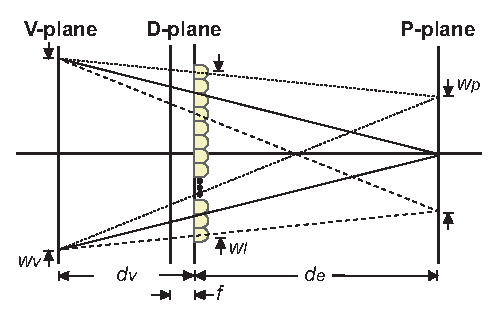
\includegraphics[width=0.95\linewidth]{images/overview_hyperopia.eps}
	\end{center}
	\caption{Geometry of the proposed framework for correcting myopia (top) and hyperopia (bottom). $D$-plane: light field display plane, $V$-plane: the virtual image plane, and $P$-plane: the eye's pupil plane}
\label{fig:overview}
\end{figure}

Following the notion of Zwicker~\etal~\cite{zwicker2006antialiasing}, let us suppose the light field display has angular and spatial sample space as $\Delta v$ and $\Delta t$, respectively. In Figure~\ref{fig:overview}, we explained angular and spatial resolutions of the light field display using microlens (or lenslet) array, which is placed a focal distance $f$ in front of the 2D display. Note that, various types of light field display (\ie, pin-hole array) are adoptable to the proposed system.

Field of view (FOV), which indicates the extent of the observable image through the display, is limited by widths of the virtual image ($w_v$) and the display ($w_d$).
\[ \text{FOV} =
  \begin{cases}
    2\arctan\Big(\min\Big[\frac{w_l}{2d_e}, \frac{w_v}{2(d_e-d_v)}\Big]\Big)  & \quad \text{for myopia}\\
    2\arctan\Big(\min\Big[\frac{w_l}{2d_e}, \frac{w_v}{2(d_e+d_v)}\Big]\Big)  & \quad \text{for hyperopia}\\
  \end{cases}
\]

%\begin{equation}
%\textsc{FOV} = 2\arctan\Big(\min\Big[\frac{w_l}{2d_e}, \frac{w_v}{2(d_v+d_e)}\Big]\Big)
%\end{equation}

%The magnification of the virtual image depends on the distance $d_v$ and the width of display $w_d$.

%\begin{equation}
%M = \frac{w_d}{d_e} \times (d_e-d_v-f)
%\end{equation}

\subsubsection{Spatial and Angular Resolution Requirements}
For light field rendering of 2D object placed at the constant depth, Chai~\etal~\cite{chai00} have shown the maximum spatial resolution for light fields reconstruction of object without aliasing can be determined by the following two factors: the angular resolution and the spatial sampling rate of the virtual image ($\Delta s$). Given an virtual image placed $d_v$ from the display, the maximum spatial spacing can be derived as follows:
\begin{equation}
\Delta t_{\max} = d_v \max( \Delta v, 2\Delta s )/f
\end{equation}
Note that, $\Delta s$ should be bounded by the highest spatial sampling rate of human retinal vision $\Delta u~(\leq \Delta s)$, which is approximately one cycle per arcmin [REF!]. Pamplona~\etal~\cite{pamplona12} has shown the required pixel pitch of displays that matches to the maximum human retinal resolution. As mentioned in Chai~\etal, if we can remove high frequency components of 2D object by applying low-pass filtering, which satisfies $\Delta s > 2\Delta v$, and the equation can be reduced as follows:
\begin{equation}
\Delta t_{\max} = d_v \Delta v/f 
\label{eq:resolutionLimits}
\end{equation}
To satisfy the condition $\Delta s > 2\Delta v$, $w_v$ should be larger than $2fw_d/d_v$ (for the proof, see supplemental materials). According to Zwicker~\etal, light fields can be rendered maximizing the use of spatial resolution of display if it satisfies $|d_v| \leq f\Delta t/\Delta v$. This indicates a virtual image placed farther than $f\Delta t/\Delta v$ will be rendered blurred.

% consider human eye resolution limit (1 arcmin), which gives the min of an object size
% also set limit to the max viewing zone

\subsection{Light Field Rendering}
Ray tracing techniques~\cite{glassner1989introduction} in computer graphics are applied to light field signal simulation. As illustrated in Figure \ref{fig:overview}, every ray is traced from the LCD plane to the pinhole plane, and then intersected with the virtual plane to be assigned the intensity of the intersected pixel. We used the Monte Carlo integration method in our ray tracing scheme.

When the distance between viewer and display is large, we can assume rays entering the pupil in parallel. There will be no cross talk between neighboring pinholes (or micro-lens) as long as the viewer moves within a viewing zone determined by the angular resolution of the display. However, when the distance between viewer and the display is small, the assumption of parallel rays no longer holds and there will be cross talk. Cross talk happens when rays entering the eye from oblique angles that were not captured by the light field signal. Figure \ref{fig:crosstalkDisplay}a shows cross-talk in terms of ray space representation. The dashed areas correspond to cross-talk rays that are not considered during light field signal simulation, and thus are not represented by the display.

To avoid Cross-talk that often results in undesirable warping effect, we consider the viewing point to be local and re-center each bloack of sensor pixels underneath each pinhole. In ray space, this corresponds to a pre-shearing of the display, as shown in Figure \ref{fig:crosstalkDisplay}b. This guarantees a cross-talk-free display when viewing point is local within the viewing zone.

\begin{figure}[t]
	    \begin{center}
   		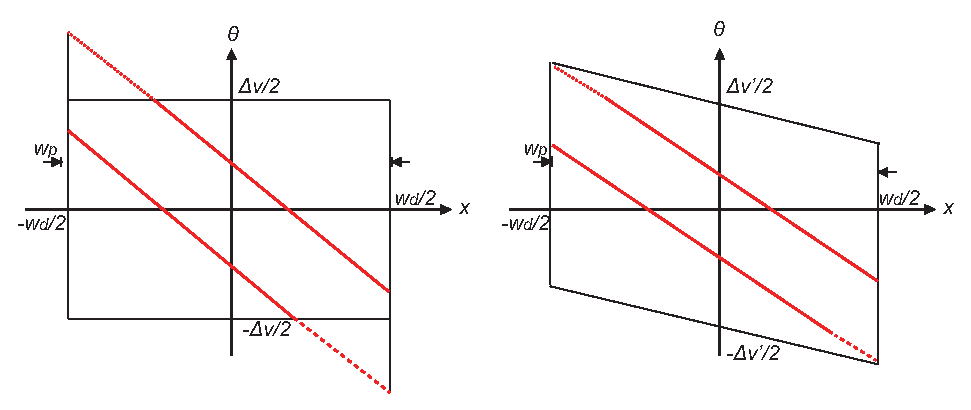
\includegraphics[width=0.95\linewidth]{images/CrossTalk.eps}
	    \end{center}
	\caption{Ray space diagram of display and eye. Left: Display with cross-talk; the dashed line corresponds to rays that are not captured by the display. Right: Pre-sheared display that takes oblique angled rays into consideration in order to avoid cross-talk.}
\label{fig:crosstalkDisplay}
\end{figure}

\begin{figure}
    \begin{center}
        \fbox{\rule{0pt}{2in} \rule{.45\linewidth}{0pt}}
    \end{center}
    \caption{Ray-space diagrams for higher-order aberration will appear here}
    \label{fig:rayspace_highorderaberration}
\end{figure}




%-------------------------------------------------------------------------
\section{Analysis}
\begin{figure}[t]
	    \begin{center}
		%\fbox{\rule{0pt}{2in} \rule{0.9\linewidth}{0pt}}
   		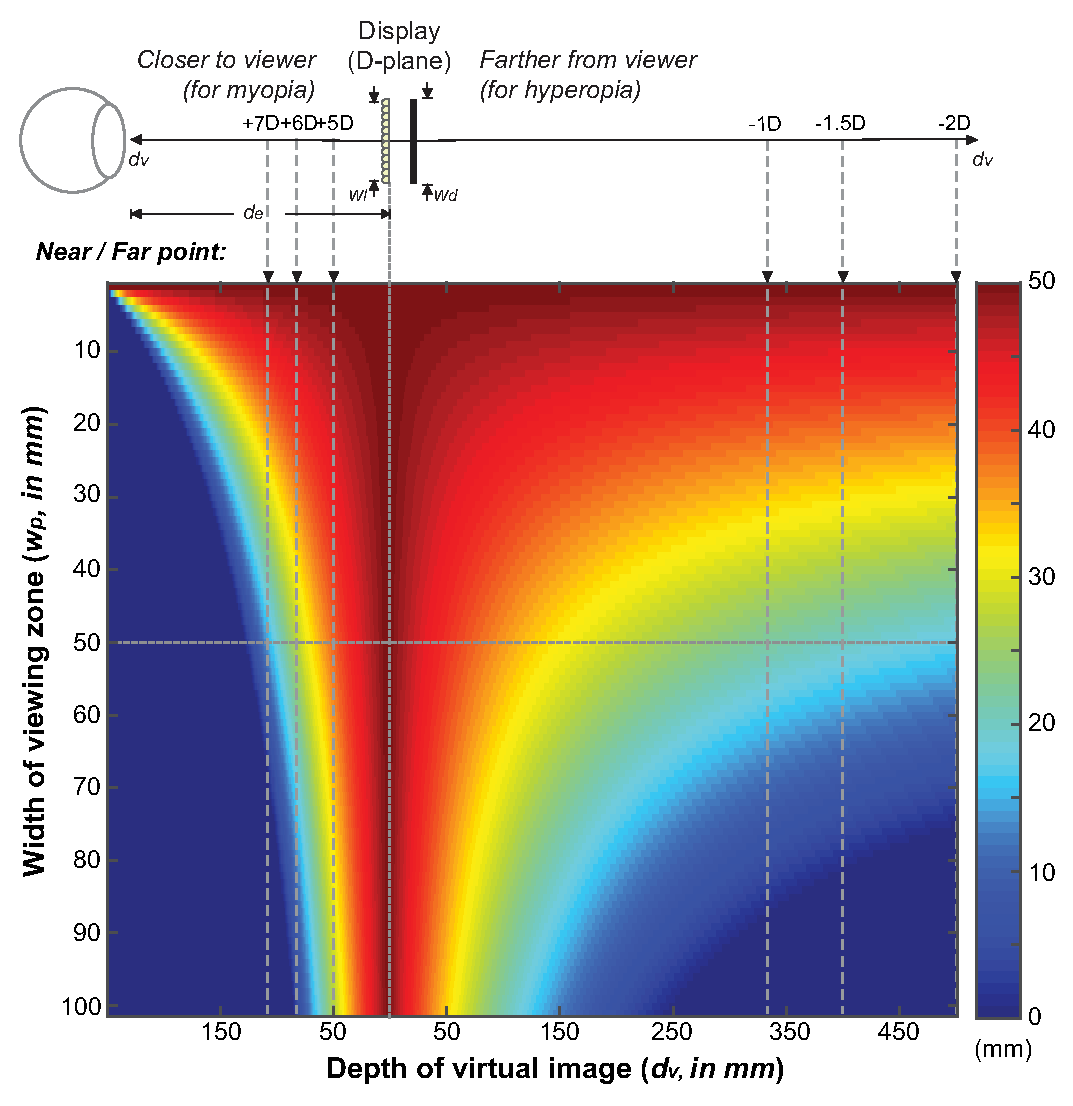
\includegraphics[width=0.90\linewidth]{images/viewingZ_v3.eps}
	    \end{center}
	\caption{(a) The size of perceived virtual image in terms of the width of viewing zone ($w_p$) and the depth of virtual image ($d_v$). Display with the width of display $w_d(=100mm)$ is placed $d_e(=250mm)$ from the viewer.}
\label{fig:viewingZone}
\end{figure}

For the sake of explanation, let us suppose the following viewing environment. As shown in Figure~\ref{fig:viewingZone} (top), a viewer is seeing a 1D display, which has the width $w_l(=50mm)$ and is placed $d_v(=250mm)$ in front of the viewer. 

\subsection{Widths of viewing zone and virtual image}
In Figure~\ref{fig:viewingZone}, the widths of perceived virtual image are shown in terms of two dependent factors: the width of viewing zone ($w_p$) and the depth of virtual image ($d_v$). We also depicted locations of near points (for hyperopia) and far points (for myopia) as dotted vertical line. The maximum size of perceived virtual image is bounded by the size of display ($w_d=50mm$). Note that, optical correction for myopic eyes with $0$ to $+4$ diopter is not required, since the image on display comes to focus on retina without any effect of blurring. With fixed viewing position ($w_p=0$), the size of perceived virtual image is same as the width of display, while the size decreases as more freedom in the viewing point is given. 

\begin{figure}
    \begin{center}
    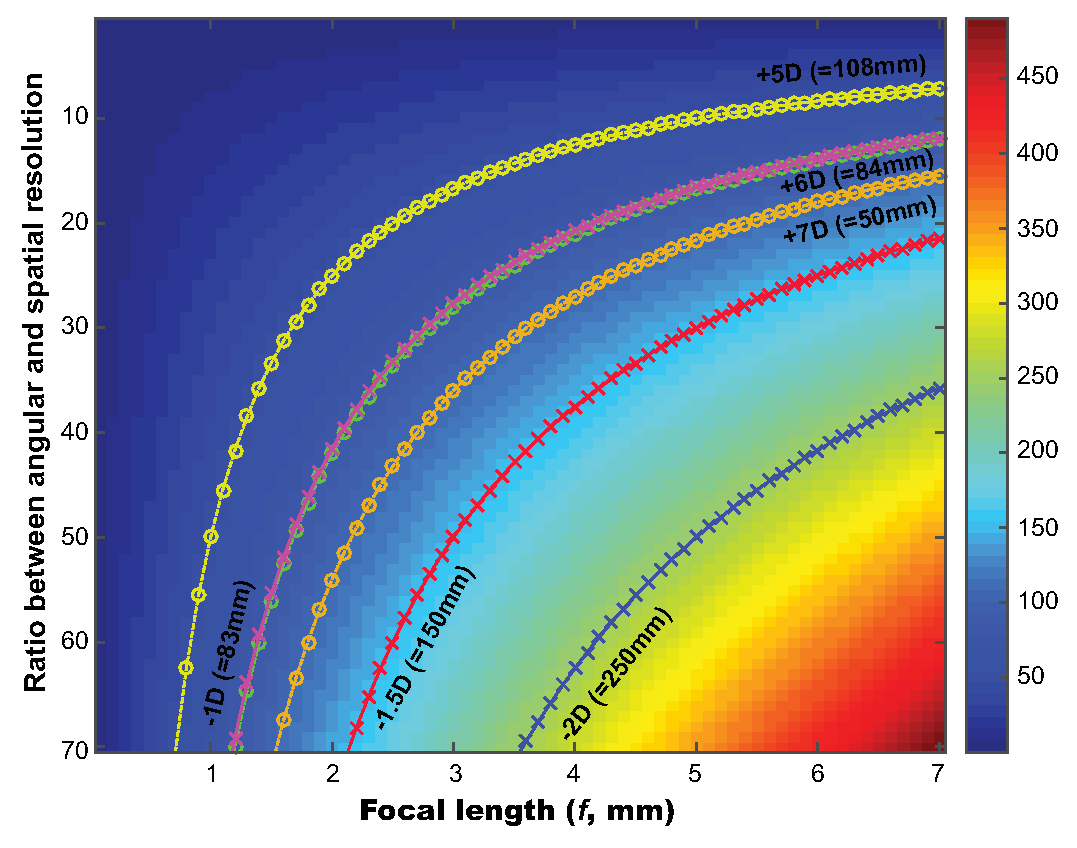
\includegraphics[width=0.95\linewidth]{images/resolutionLimits_v2.eps}
    \end{center}
    \caption{Spatial and Angular resolution limits}
    \label{fig:resolutionLimits}
\end{figure}

\subsection{Spatial and Angular Resolution Limits}
In Figure~\ref{fig:resolutionLimits}, we illustrate the maximum distance at which a virtual image can be placed, maximizing the use of spatial resolution of display based on Equation~\ref{eq:resolutionLimits}. We draw the figure in terms of two parameters: the ratio between angular and spatial resolution ($=\Delta t / \Delta v$) and the focal length ($f$). As expected, as both parameters increase, a farther virtual image can be rendered. Each line in the figure represents the minimum required system setting for correcting eye-aberration (\ie, +5D to +7D for myopia, -1D to -2D for hyperopia).

\subsection{Eye Correction limits}
According to the anti-aliasing display analysis by Zwicker\etal~\cite{zwicker2006antialiasing}, given a display with spatial sample spacing of $\Delta t$ and angular sample spacing $\Delta v$, the maximum plane depth where the scene can be represented with full spatial resolution of the display is $|z| = \Delta t / \Delta v$, where $z$ is the distance between the focal plane and the display. As there is a one-to-one mapping between depth of focal plane and eye aberration (in diopter D, given in mm), this depth limit sets a constraint on the correction power of a display with a fixed spatial and angular resolution. The limitation of eye aberration that can be corrected by a display with $\Delta t$ and $\Delta v$ is:
$$D = \frac{1000}{d_e-\Delta t / \Delta v}$$
where $d_e$ is the distance between viewer and display. More intuitively, for the screen size of an iPhone 6s (120 mm diagonal) and a normal viewing distance of 250 mm, in order to correct a myopic eye with -2D aberration, we require a the virtual image plane to be placed 200 mm behind (away from the viewer) the display.

\subsection{Higher order aberration} \label{ss:Higherorderaberration}
Any type of viewing-independent vision-correcting display that supports free eye-movement would create error in correcting higher-order aberration, which includes coma, astigmatism, distortion, and spherical aberration. To prove it, suppose that $N$ parallel light rays $l_i$ ($i=1,2,...,N$) is coming from the virtual plane to the eye's pupil plane, and each ray is uniformly spaced by $\Delta h$, which is sufficiently smaller than the size of eye's entrance pupil. Given any types of aberration, light rays entering eye's entrance pupil would create transverse error $\epsilon_i$. Now, let us assume the eye is moving in lateral direction with an amount larger than $\Delta h$. If there appears a non-linear variation in transverse error difference (\ie, $|\epsilon_i -\epsilon_{i-1}|$), light fields should be recalculated based on the position of eye for accurate correction. Unlike low-order aberrations (\ie, myopia and hyperopia) that produce a constant transverse error difference between neighboring light rays, higher-order aberrations have transverse error that would vary periodically (see supplemental material for more details). This introduces difficulties to make the viewing-independent vision-correcting display for higher-order aberration. In Figure~\ref{fig:rayspace_highorderaberration}, we illustrate ray space diagram for 4 major types of high-order aberration: coma, astigmatism, distortion, and spherical aberration. 




%-------------------------------------------------------------------------
\section{Result}
\subsection{Retinal Image Simulation}
To demonstrate the effect of the proposed method, we implemented a retinal image simulator that constructs a projection matrix between pixels on display and sampled sensor points on retina based on ray-tracing. To this end, we employed the model of Seidel aberration~\cite{wyant92} to calculate transverse aberration as follows:
\begin{equation}
\epsilon_x = -\frac{R}{n'e'}W_{020}\rho_x,~~ \epsilon_y = -\frac{R}{n'e'}W_{020}\rho_y
\end{equation}
where $n'$ is refractive index of eye, and $R$ indicates the radius of curvature of the spherical wavefront, while $e'$ denotes the semi-aperture of the exit pupil. $\rho_x$ and $\rho_y$ represent the exit pupil coordinates represented in polar coordinates. Depending on the level of optical defocus aberration, $W_{020}$ can be determined. (For more details, see \cite{wyant92})


\subsection{Eye movement-free correction}




%-------------------------------------------------------------------------
\section{Discussion}
\subsection{Limitations}


\subsection{Future work}

%higher order aberration approximation?
% talk about multiplexing to correct both eyes


%-------------------------------------------------------------------------
\section{Conclusion}

%-------------------------------------------------------------------------
%{\small
\bibliographystyle{ieee}
\bibliography{vcd}
%}

\end{document}
